\subsection{Extraction of the $\Zmm$ signal yield \label{sec:Zmumu}}

%$\Zmm$ are characterized by the presence of two high-pt isolated muons.
We extract the $\Zmm$ cross-section on the basis of a simultaneous
Poissonian likelihood ratio fit of the yield of $\Zmm$ event,
the average reconstruction muon 
efficiencies in the tracker and in the muon detector, the trigger efficiency, 
as well as the efficiency isolation cut
.%The extracted $Z$ yield has to be corrected only for the geometrical acceptance and for
%the integrated luminosity in order to determine the cross section.
We consider events with two muon candidates with $\Pt>20$~GeV$/c$ and $|\eta|<2.1$
in the di-muon mass range from 60 to 120 GeV$/c^2$.
where muon candidates can be detected in either or both the tracker and
muon detector. Muons are checked for matching with HLT objects.
We don't use calorimeter information in the definition of isolation 
order not to correlate isolation with the presence of final-state photons.
%, and
%we require that the muons are isolated if $\sum (\Pt(tracks)) < 3.0$~$\mathrm{GeV}/c$.
The muon quality cut on $\chi^2/{\mathrm{ndof}}$ and 
the request that the muon is found by the tracker algorithm are
dropped to minimize the tracker and muon detector efficiency correlation.
% We require that a tracker track has
% at least 11 tracker hits (pixel + silicon tracker layers) and at least 1 pixel hit,
% consistently with the muon selection criteria.
% In addition, we require that the stand-alone muon track should have at least 1 muon hit and
% at least 2 segments matched to the muon track. 
%The efficiencies of these additional selection cuts are incorporated in the
%reconstruction efficiency terms.
We build five statistically independent event categories with muons
passing or failing the reconstruction in either the muon detector and/or tracker,
the trigger matching and/or the isolation cut.
The signal yield in the four categories can be rewritten in terms of the
number of produced $\Zmm$ events, $\NZtomumu$, and the average efficiencies 
for muon reconstruction in the tracker ($\effTrk$), in the muon detector
($\effSa$), the average efficiency of the isolation 
cut ($\effIso$) and the average trigger efficiency ($\effHlt$),
where the efficiency of the muon quality cuts are incorporated in the definition
of $\effTrk$ and $\effSa$.
%
% \begin{eqnarray}
%  \label{eqNmumuTwoHlt}
%    \NmumuTwoHlt & = & \NZtomumu \effHlt^2 \effIso^2 \effTrk^2 \effSa^2,  \\
%   \label{eqNmumuOneHlt}
%    \NmumuOneHlt & = & 2 \NZtomumu \effHlt (1 - \effHlt) \effIso^2 \effTrk^2 \effSa^2,  \\
%   \label{eqNmus}
%    \Nmus & = & 2 \NZtomumu \effHlt \effIso^2 \effTrk (1 - \effTrk) \effSa^2,  \\
%   \label{eqNmut}
%    \Nmut & = & 2 \NZtomumu \effHlt \effIso^2 \effTrk^2 \effSa(1 -\effSa), \\
%   \label{eqNmumuNonIso}
%    \NmumuNonIso & = & 2 \NZtomumu \effHlt^2  \effIso (1 - \effIso)  \effTrk^2 \effSa^2. 
% \end{eqnarray}
% The efficiency $\effTrk$, which appears in the
% equations (\ref{eqNmumuTwoHlt}-\ref{eqNmumuNonIso}) is
% the efficiency to reconstruct a track {\it and} to pass the two additional 
% efficiencies $\effTrk \rightarrow \effTrk \times
% \epsilon_{\mathrm{\#TrackerHits}>10} \times \epsilon_{\mathrm{\#PixelHits}>0}$. 
% $\effSa$ is the efficiency to reconstruct a
% stand-alone track {\it and} to pass the two additional efficiencies $\effSa
% \rightarrow \effSa \times \epsilon_{\mathrm{\# MuonHits}>0} \times \epsilon_{\mathrm{\#Matches}>1}$. 
The background expected in the event categories with two muons 
reconstructed in both the tracker and muon detector (``golden'' event) 
is negligible, and we use only the number of events in such categories in the simultaneous fit.
We use the di-muon invariant mass spectrum from the ``golden'' events as 
template for all categories, except the one with one muon reconstructed in the muon detector only,
which has a significantly worse resolution than the tracker alone,
for  $\Pt\leq 200$~GeV. In that case, we take the ``golden'' di-muon 
spectrum considering, for one of the two muons, the momentum measured in the 
muon detector only.
The background in the non-golden categories is modeled as the product
of an exponential times a polynomial.


% Background functions are modeled as products of exponential terms with polynomials 
% of different order for the three samples for which the background is not neglected:
% \begin{eqnarray}
%   b_{\mu t}(m) & = & N^b_{\mu t} (1 + a_1 m + a_2 m^2) e^{-\alpha m} \\
%   b_{\mu\mu}^{\mathrm{non\,iso}}(m) & = &
%   N_{\mu\mu}^{b\,\,{\mathrm{non\,iso}}} (1 + b_1 m + b_2 m^2) e^{-\beta m} \\
%   b_{\mu s}(m) & = & N^b_{\mu s} (1 + c_1 m + c_2 m^2) e^{-\gamma m} 
% \end{eqnarray}
% We also tried different background models and different binning size for the 
% categories different from $\Zmumu$ and determine fit systematic uncertainty accordingly.

%  f_{peak}^{s}(m) & = & \frac{1}{\sqrt{2\pi\sigma_s^2}} e^{-\frac{(m - M)^2}{2 \sigma_s^2} } \\
%The peak function for the $\Zmus$ category, $f_{peak}^{s}(m)$, is modelled as a
%Gaussian, due to the poor resolution, and the low statistics in that sample:

% We divide the invariant di-muon mass spectrum of the different categories into
% bins whose size depends on the statistics of each of the five categories. 
% We define, for each category, minus two times the negative logarithmic
% of the following Poissonian likelihood ratio~\cite{PoisLR}:
% \begin{equation}
% \chi^2_{\lambda} = -2 \ln{\lambda(m)} =  -2 \ln{\frac{\mathrm{Poiss}(n_i,
%     \nu_i)}{\mathrm{Poiss}(n_i, n_i)}} = \sum_{i=1}^{n_{\mathrm{bins}}} \nu_i - n_{i} + n_i \log{\frac{n_i}{\nu_i}}\,,
% \end{equation}
% where $\nu_i$ is the expected number of events in the $i^{\mathrm{th}}$-bin of the
% di-muon invariant mass histograms and $n_i$ is the measured number of events in that
% bin, and $\mathrm{Poiss}(n,\nu)$ is a Poissonian distribution.
% In ordr to perform the simultaneous fit, we minimize the
% sum $R$ of the five $\chi^2_\lambda$, i.e.: 
% \begin{equation}
% R =  \sum_{j=1}^{5} \chi^2_{\lambda,j}   = 2  \sum_{j=1}^{5} \sum_{i=1}^{n_{\mathrm{bins}}^{(j)}} \nu^{(j)}_i - n^{(j)}_{i} + n^{(j)}_i \log{\frac{n^{(j)}_i}{\nu^{(j)}_i}}\,, 
% \end{equation}
% where the index $j$ runs on the five categories, and the index $i$ on the bins of
% the $j^{\mathrm{th}}$ category.
% A benefit of this statistic technique is that it allows a
% goodness-of-fit test, as for sufficiently large $\nu_i$ the minimum of $R$ follows a $\chi^2$ distribution.
% Using a single bin (counting only) and a Gaussian approximation for the two categories with the largest statistics, $\ZmumuTwoHlt$ and $\ZmumuOneHlt$,
% the Z yield and the four efficiencies are obtained by minimizing:
% \begin{eqnarray*} \label{chi2}
% R & = &  
% \frac{(\NmumuTwoHlt - \NZtomumu\effHlt^2\effIso^2\effTrk^2\effSa^2)^2}{\NmumuTwoHlt} +  \\
% & & \frac{(\NmumuOneHlt - 2\NZtomumu\effHlt(1-\effHlt)\effIso^2\effTrk^2\effSa^2)^2}{\NmumuOneHlt} +  \\
% & & \chi^2_{\lambda, \mu s} + 
% \chi^2_{\lambda, \mu t} + 
% \chi^{\nonIso\,\, 2}_{\lambda, \mumu}\, , 
% \end{eqnarray*} 
% where we count the events $\ZmumuOneHlt$ and $\ZmumuTwoHlt$ golden
% categories and $\chi^2_{\lambda, \mu s}$, $\chi^2_{\lambda, \mu t}$ and
% $\chi^{\nonIso\,\, 2}_{\lambda, , \mumu}$ are the
% Poisson likelihood ratio of the di-muon mass binned histograms for the
% three categories $\Zmus$, $\Zmut$, and $\ZmumuNonIso$.
% The likelihood ratio fit is equivalent to an ordinary $\chi^2$ 
% for enough large statistics and we verified that, with the current data sample,
% it gives the same central value and statistical uncertainty.
% We perform the fit in the range $60 < m < 120~\mathrm{GeV}/c^2$.
% Full details on the signal and background modeling assumptions and
%correlation studies are present in~\cite{CMS_AN_2010-345}.

Figure~\ref{fig:zGolden36pb} shows the di-muon invariant mass spectrum in both linear and
logarithmic scale for the \Zmm ``golden''. The spectrum is in agreement 
with the simulation.
Figure~\ref{fig:zNoGold} shows the di-muon invariant mass distribution for the remaining categories.
\begin{figure}[hbtp]
    \begin{minipage}{73mm}
      \begin{center}
        \resizebox{1.0\textwidth}{!}{{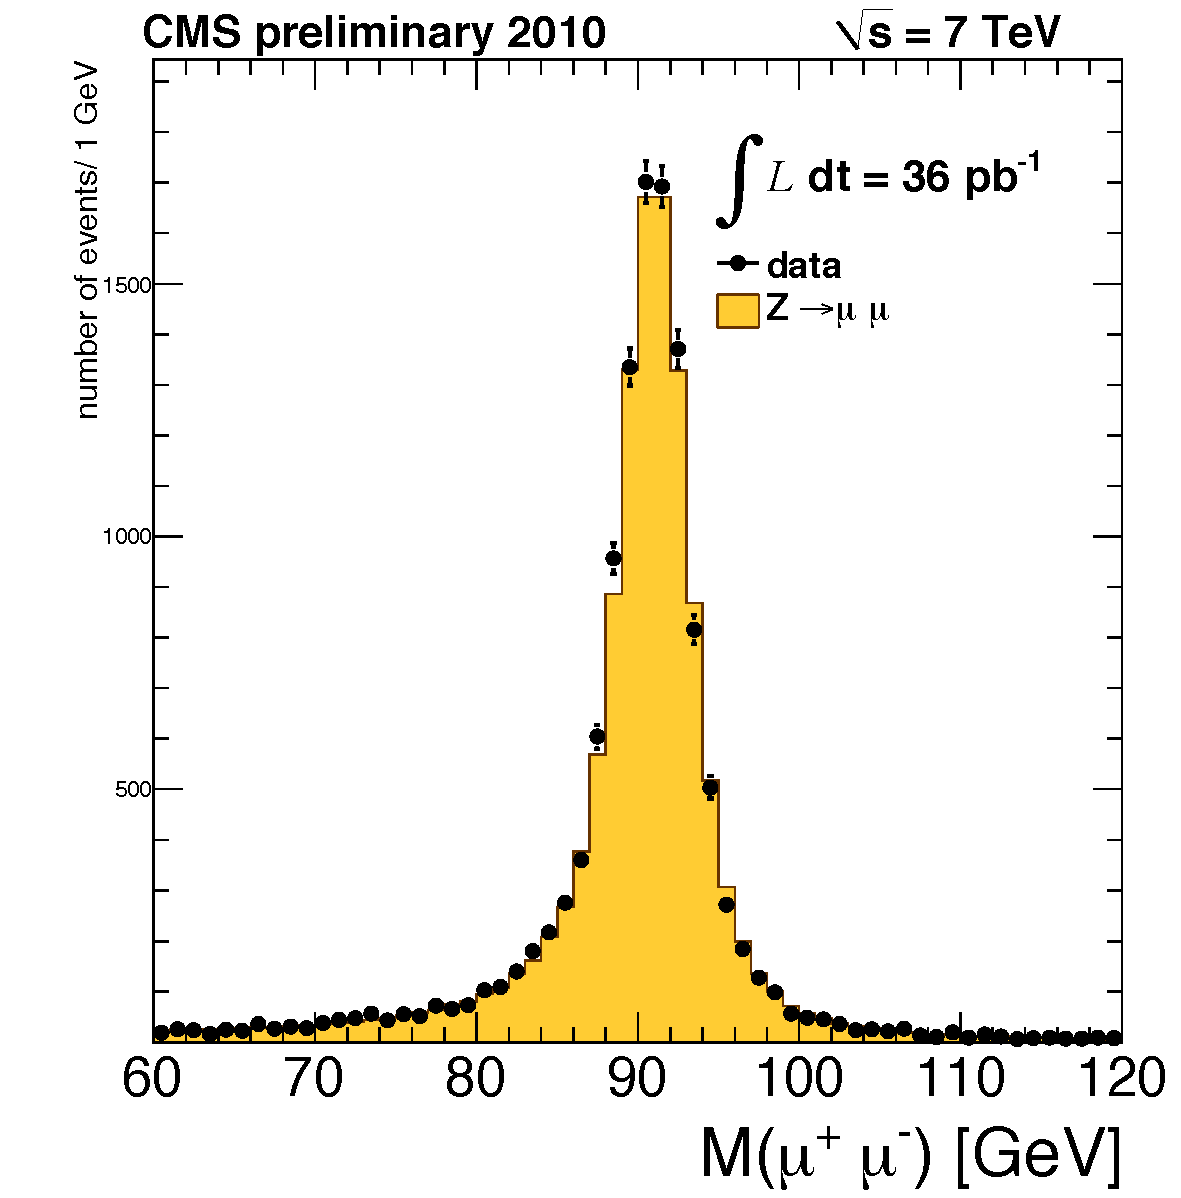
\includegraphics{figs/zGoldenLin_36pb.pdf}}}
      \end{center}
    \end{minipage}
    \begin{minipage}{73mm}
       \begin{center}
       \resizebox{!}{1.0\textwidth}{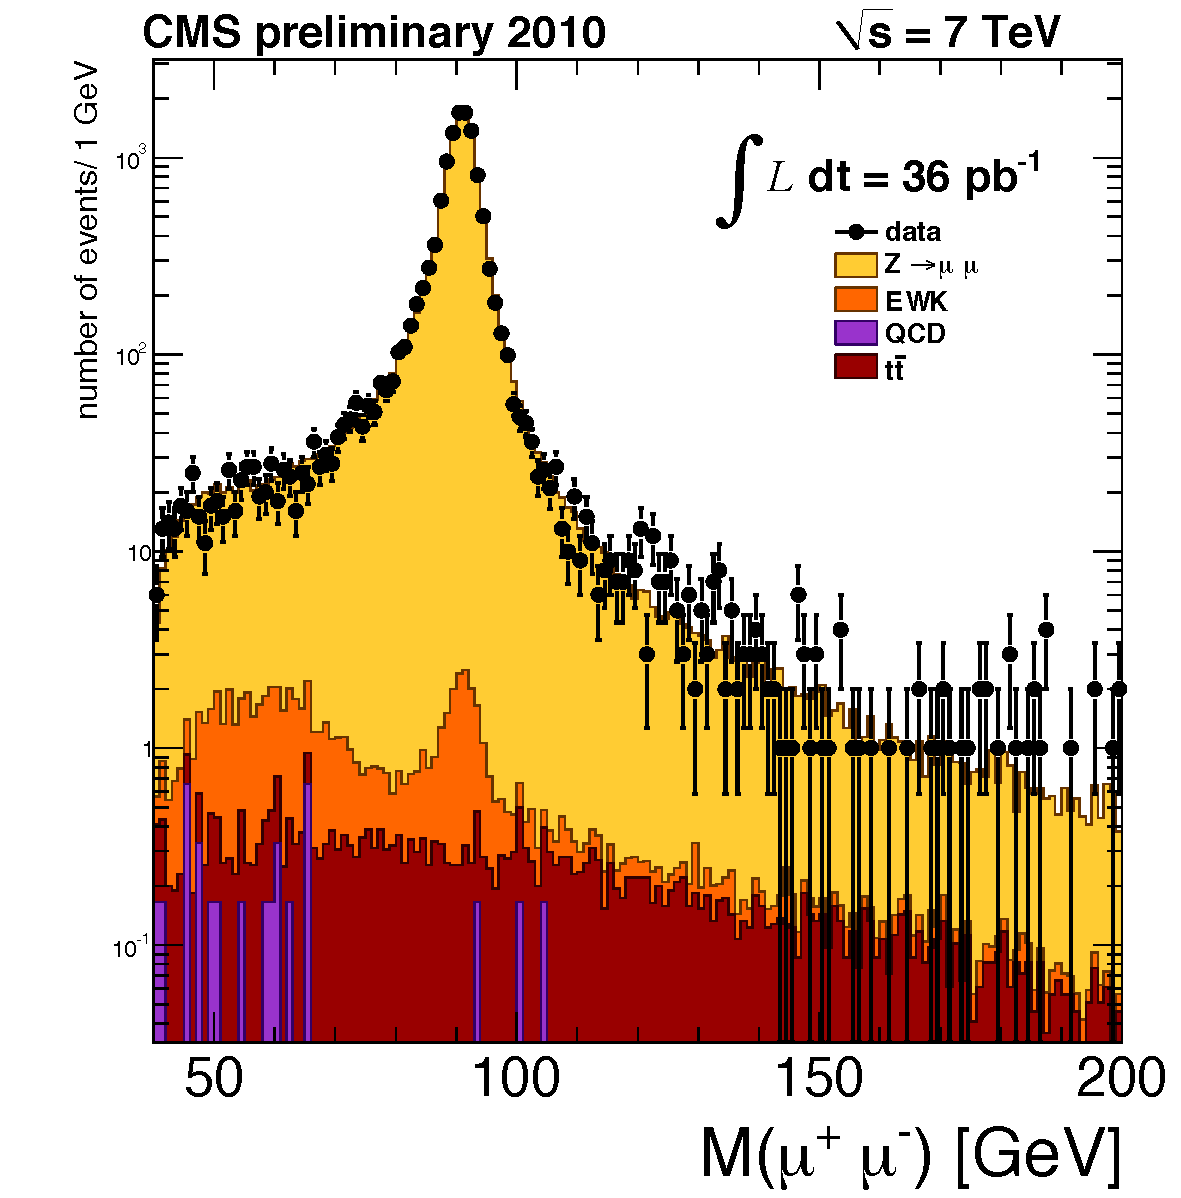
\includegraphics{figs/zGoldenLog_36pb.pdf}}
      \end{center}
    \end{minipage}
\caption{Distribution of the di-muon invariant mass of $\Zmm$ ``golden'' candidates for 
  data (dots) and Monte Carlo (histogram) signal and background events 
for  a luminosity of 36~pb$^{-1}$. The same distribution is shown in linear scale (left) and in 
logarithmic scale (right).}
\label{fig:zGolden36pb}
\end{figure} 
\begin{figure}[hbtp]
    \begin{minipage}{73mm}
      \begin{center}
        \resizebox{1.0\textwidth}{!}{{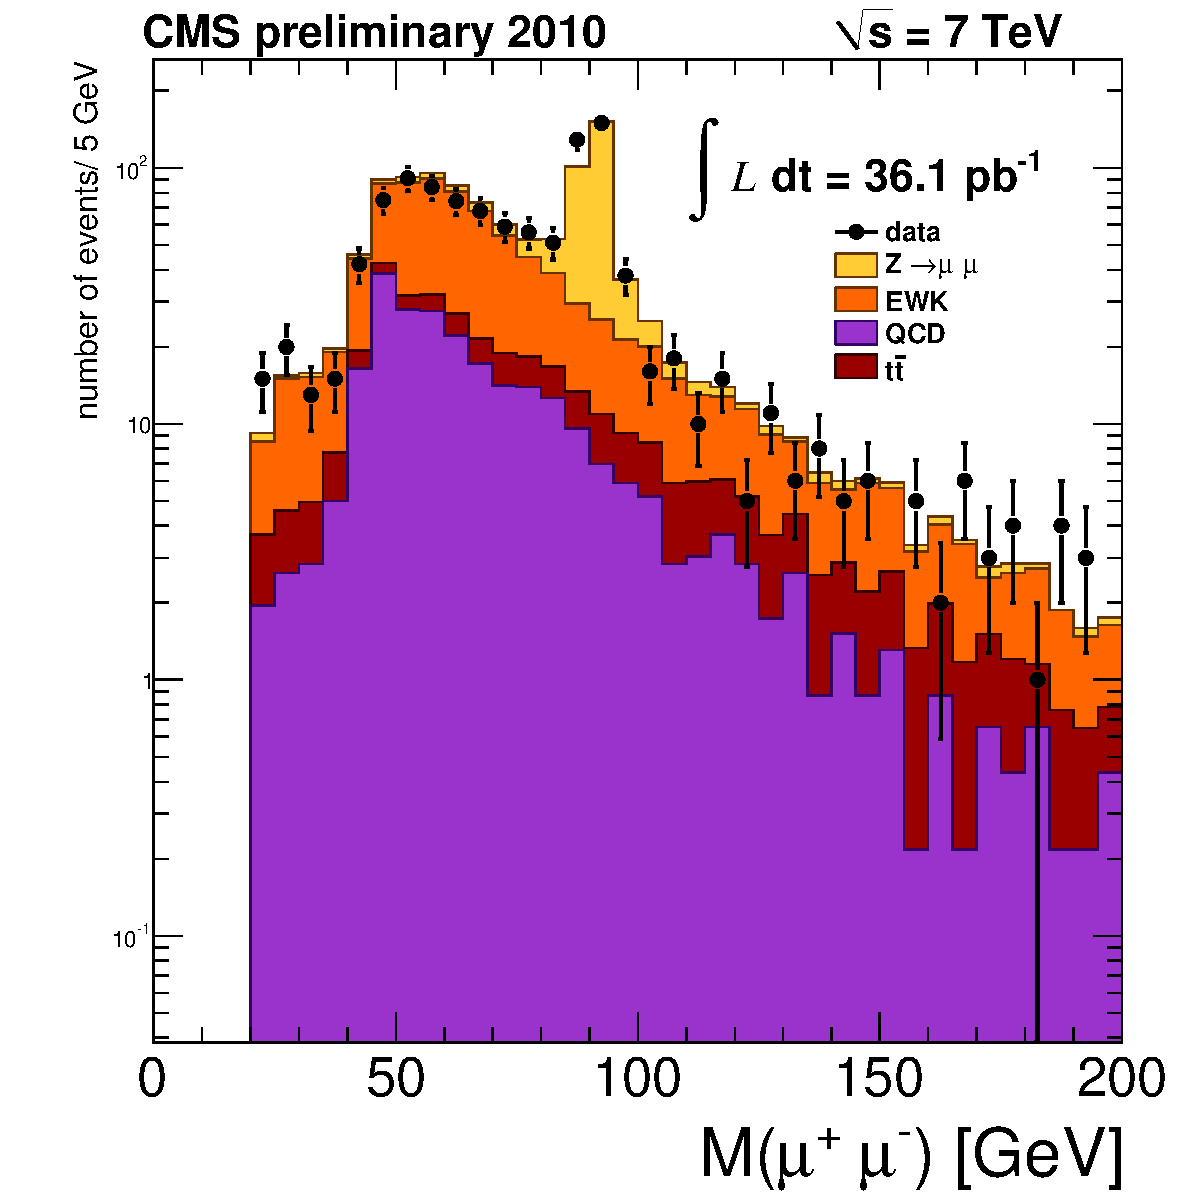
\includegraphics{figs/zMuTrk.pdf}}}
      \end{center}
    \end{minipage}
    \begin{minipage}{73mm}
       \begin{center}
       \resizebox{!}{1.0\textwidth}{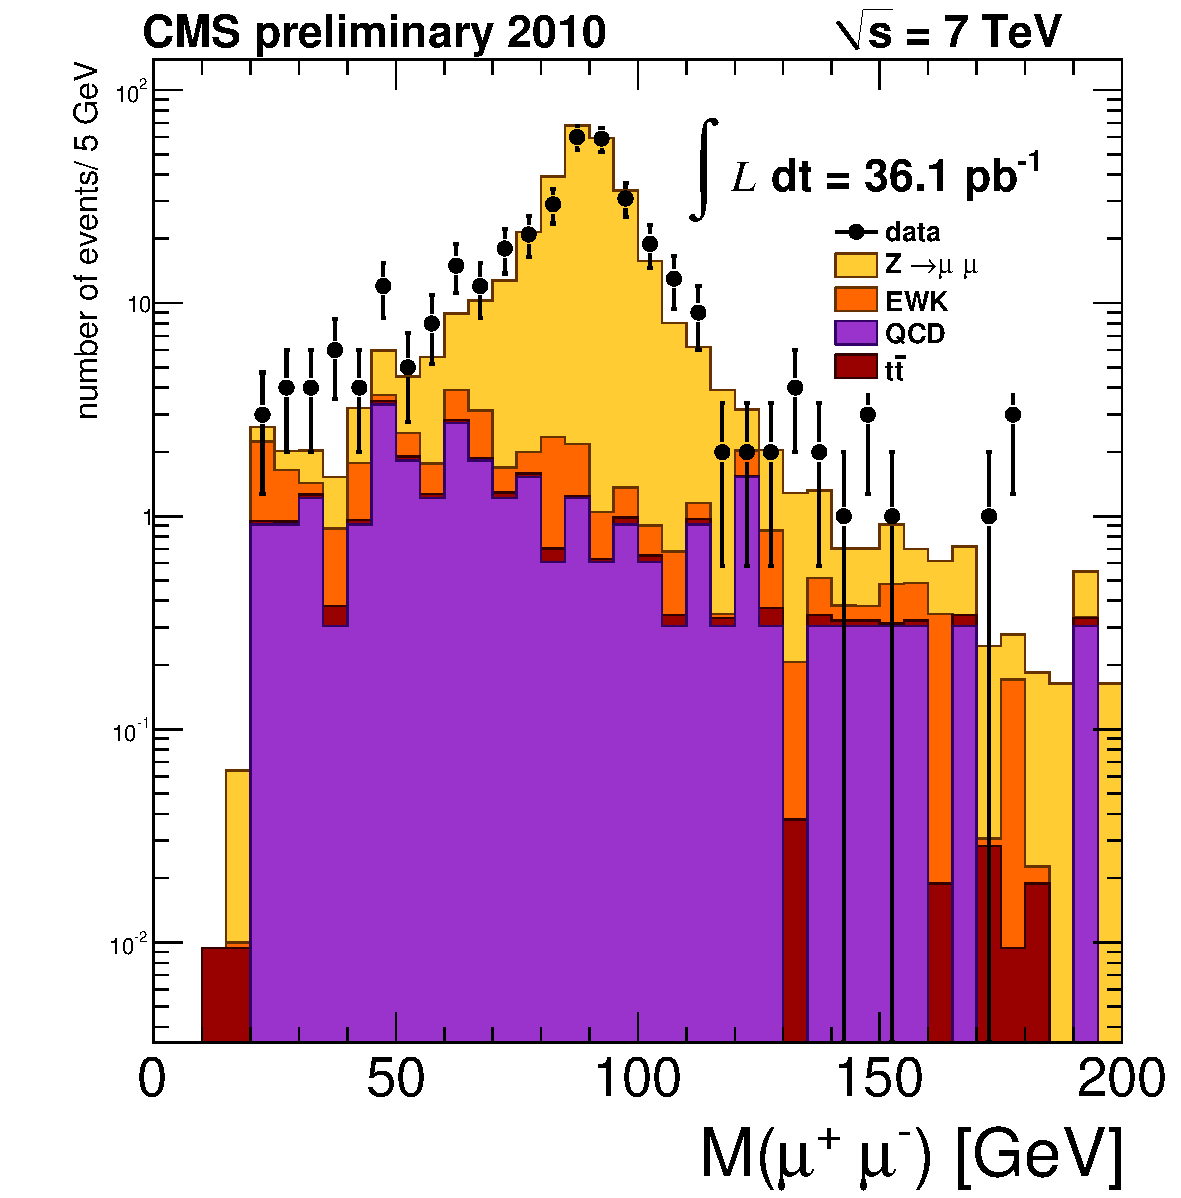
\includegraphics{figs/zMuSta.pdf}}
      \end{center}
    \end{minipage}
    \begin{center}
     \begin{minipage}{73mm}
       \begin{center}
        \resizebox{!}{1.0\textwidth}{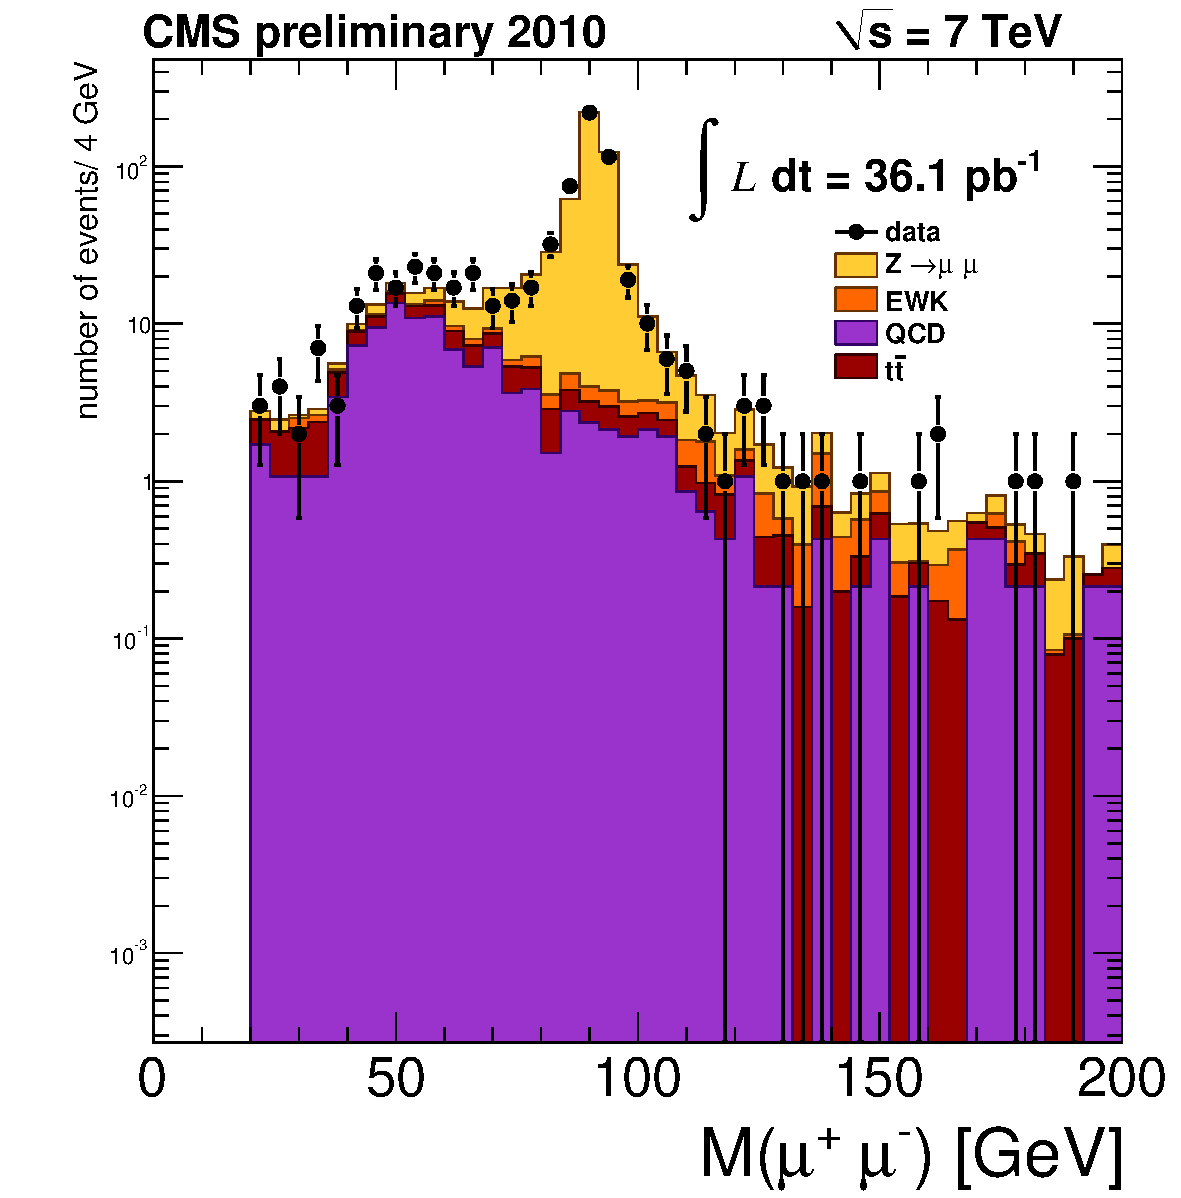
\includegraphics{figs/zOneNotIso.pdf}}
       \end{center}
     \end{minipage}
   \end{center}
\caption{Distribution of the di-muon invariant mass of $\Zmm$ candidates for 
  the  $\Zmut$ (top, left), $\Zmus$ (top, right) and $\ZmumuNonIso$ (bottom) categories.
  Data (dots) are superimposted on Monte Carlo (histogram) for signal and background normalized
to a luminosity of 36~pb$^{-1}$.}
\label{fig:zNoGold}
\end{figure} 
%Table~\ref{fig:fitRes_36pb} reports the yield and efficiencies determined from
%the fit. In addition, the Monte Carlo values of the average efficiencies for
%signal events are shown for comparison together with the correction factors (ratio of 
%data/simulation efficiencies). A good quality of the fit is measured.
%The resulting fit $\chi^2$ and correspondent $p$-value (the
%probability of obtaining a value greater that the fit $\chi^2$)
%show the good quality of the fit.
%With the analyzed statistics, a second degree polynomial function is
%taken for modelling  the background shape.

% \begin{table}[htbp]
% \begin{center}
% \begin{tabular}{|c|c|c|}
% \hline
% $\int L\mathrm{d}t = 36 \mathrm{pb}^{-1}$ & fit results on data & data/simulation\\ 
% \hline\hline
% $\effHlt$ & 0.9203$\pm$ 0.0019  &0.9672$\pm$0.0020   \\
% \hline
% $\effIso$ & 0.9813 $\pm$ 0.0010& 0.9962 $\pm$  0.0011 \\
% \hline
% $\effSa$ & 0.9762  $\pm$ 0.0012 & 0.9964$\pm$0.0013 \\
% \hline
% $\effTrk$ & 0.9890 $\pm$0.0006  & 0.9949 $\pm$ 0.0007  \\
% \hline
% $\NZtomumu$ &13728 $\pm$ 121   & \\
% %\hline
% %$\chi^2$/ndof &  1.06&\\
% %\hline
% %$p-\mathrm{value}$& 0.36 & \\
% \hline
% \end{tabular}
% \end{center}
% \caption{Comparison between fit parameters in data with simulation 
%   using the full 2010 data. $\chi^2$ divided by the number of degrees of freedom (ndof) and
%   $p$-value are also reported. Data/simulation ratio are also shown for comparison.}
% \label{fig:fitRes_36pb}
%\end{table}

% Figure~\ref{fig:zNoGold_fig} shows the fit di-muon invariant mass distribution for the
% non-golden categories.
% \begin{figure}[hbtp]
%     \begin{minipage}{78mm}
%       \begin{center}
%         \resizebox{1.0\textwidth}{!}{{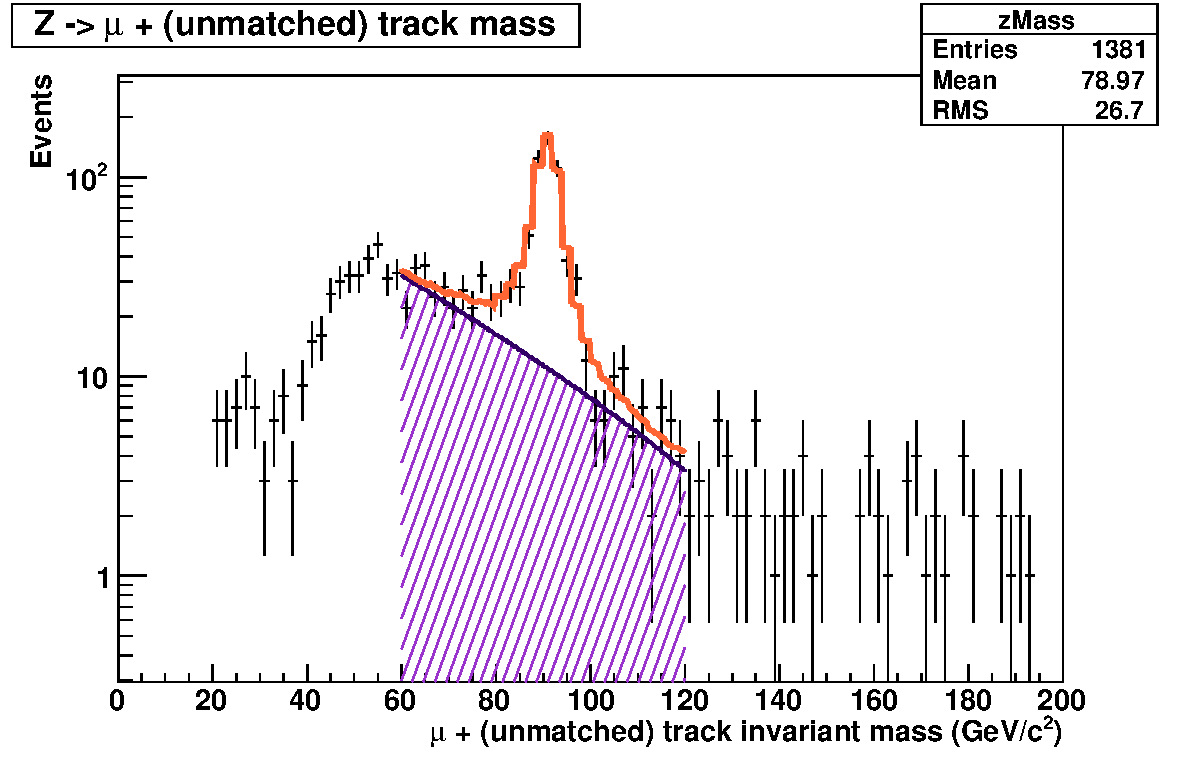
\includegraphics{figs/zMuTrk_fit.pdf}}}
%       \end{center}
%     \end{minipage}
%     \begin{minipage}{50mm}
%        \begin{center}
%        \resizebox{!}{1.0\textwidth}{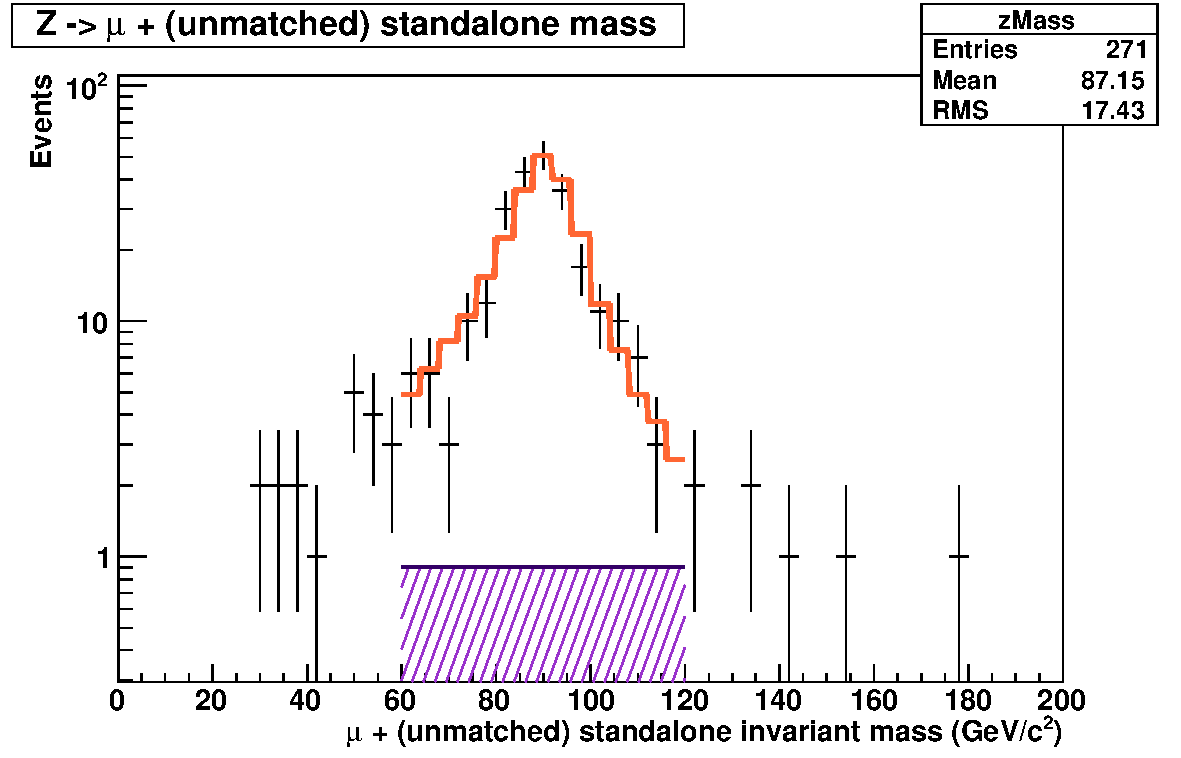
\includegraphics{figs/zMuSta_fit.pdf}}
%       \end{center}
%     \end{minipage}
%     \begin{center}
%      \begin{minipage}{50mm}
%        \begin{center}
%         \resizebox{!}{1.0\textwidth}{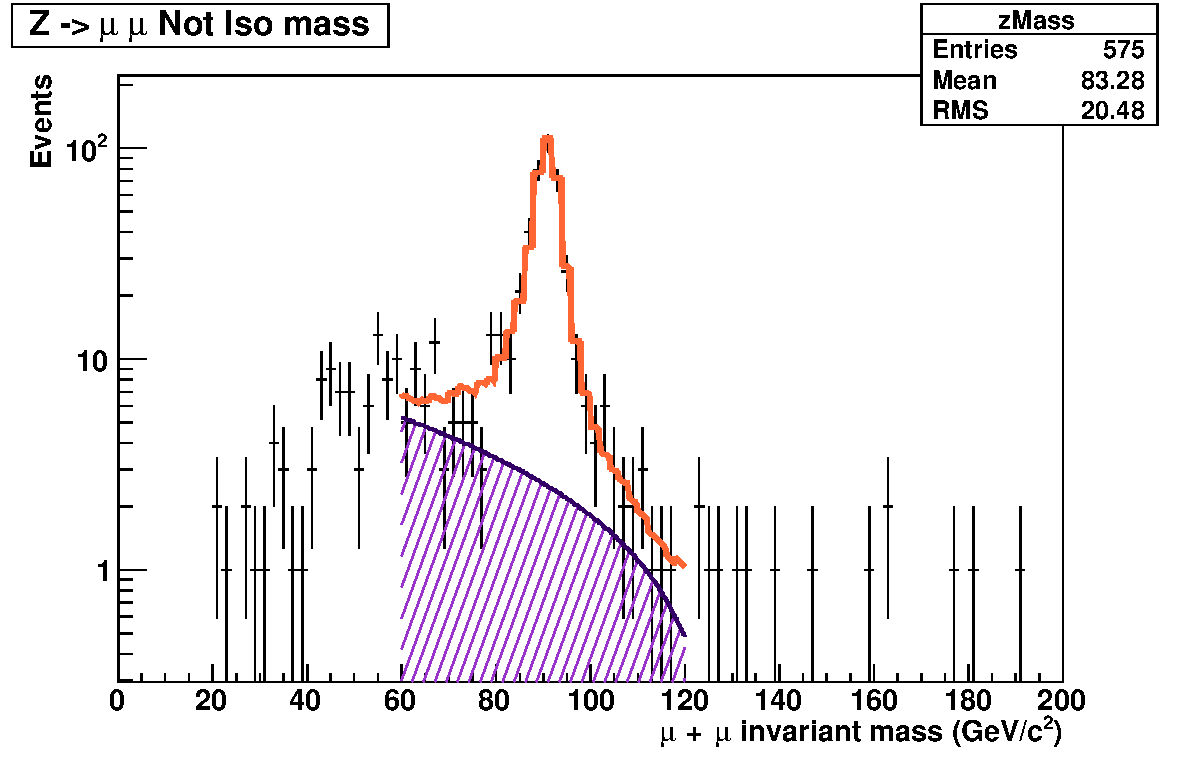
\includegraphics{figs/zOneNotIso_fit.pdf}}
%        \end{center}
%      \end{minipage}
% \end{center}
% \caption{Distribution of the di-muon invariant mass of $\Zmm$ candidates for 
%   the  $\Zmut$ (top, left), $\Zmus$ (top, right) and $\ZmumuNonIso$ (bottom)
%   categories and superimposed fit spectrum.}
% \label{fig:zNoGold_fig}
% \end{figure} 

%The $\Zmm$ yield determined from the fit corresponds to the selected kinematic range.
%In order to determine the cross section corresponding to the full phase space,
%we need to correct by the acceptance of the kinematic selection, including the
%the invariant mass range $60<m_{\mu^+\mu^-}<120$~$\mathrm{GeV}/c^2$ used in the fit.,

We estimate the acceptance using POWHEG $\Zmm$ Monte Carlo sample to be
$\epsilon^{\mathrm{kin}} = 0.3977 \pm 0.0017$
The error is statistical only.
The expected contamination fraction of irreducible background
is $f_{bkg}=0.43 \pm 0.02\%$. We subtract this fraction and take the
uncertainty as systematic error.

% Table~\ref{tab:zmmBkg} reports the number of expected
% events from different sources of background.

% \begin{table}[htbp]
% \begin{center}
% \begin{tabular}{|c|c|c|}
% \hline
% source & events \\
% \hline\hline
% Electro-weak (other and Z) & $37\pm1$ \\
% $\ttbar$ & $18\pm 2$ \\
% QCD & $1.7\pm0.1$ \\
% \hline
% Total & $55\pm 3$\\
% \hline
% \end{tabular}
% \end{center}
% \caption{Expected number of background events with the collected luminosity from various
% background sources in the di-muon mass range from 60 to 120~GeV.}
% \label{tab:zmmBkg}
% \end{table}